\chapter{Pipelining}

\section{Introduzione e Concetti Base}
Il \textbf{pipelining} è una tecnica di implementazione in cui l'esecuzione di più istruzioni viene sovrapposta nel tempo. 
In una pipeline, diverse unità hardware (chiamate \textit{stadi della pipeline} o \textit{segmenti}) completano parti diverse di istruzioni distinte in parallelo.

% FIGURA DA INSERIRE QUI
% Fonte: Slide 3
% Descrizione: Schema temporale semplificato che mostra l'overlapping delle fasi F (Fetch), D (Decode), E (Execute), W (Write-back) per 4 istruzioni nei cicli di clock.
\begin{figure}[H]
    \centering
    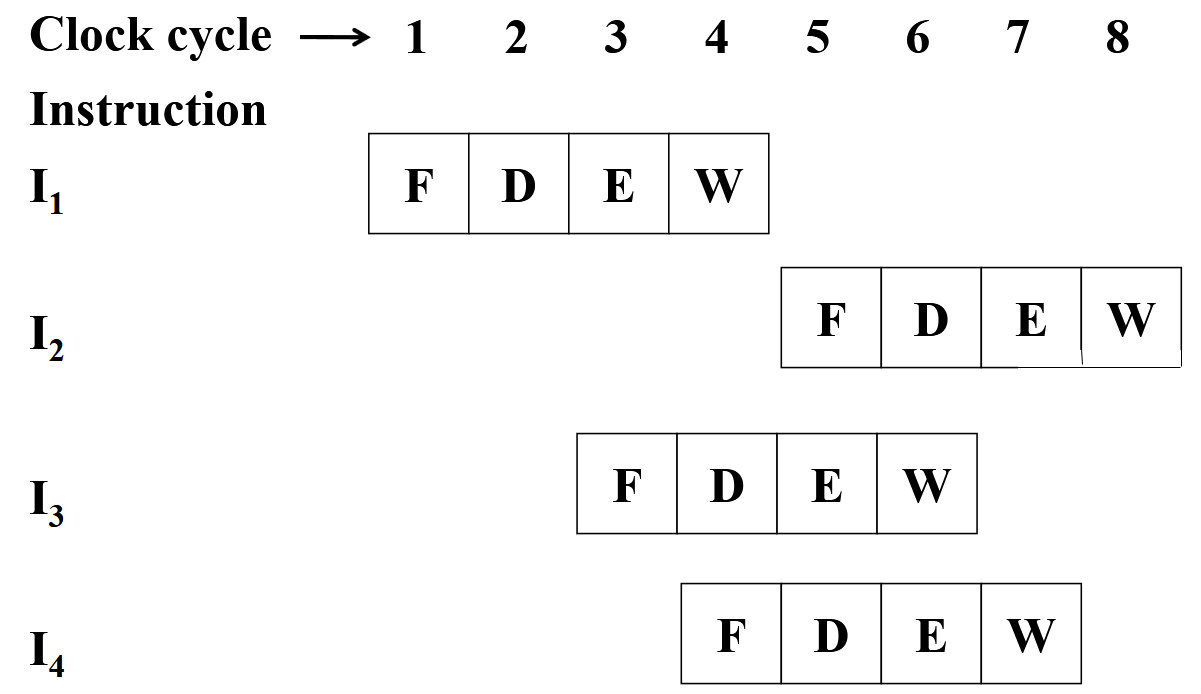
\includegraphics[width=0.5\textwidth]{capitoli/05_pipelining_base/images/overlapping_fdew.png}
    \caption{Sovrapposizione dell'esecuzione delle istruzioni nei vari cicli di clock.}
    \label{fig:pipeline_intro}
\end{figure}

\subsection{Definizioni Fondamentali}
\begin{itemize}
    \item \textbf{Throughput}: In un processore con pipeline, il throughput è il numero di istruzioni che completano il loro percorso (ed escono dalla pipeline) nell'unità di tempo. L'obiettivo del pipelining è proprio aumentare il throughput complessivo, non velocizzare la singola istruzione.
    \item \textbf{Sincronizzazione degli stadi}: Tutti gli stadi della pipeline sono sincronizzati. Questo significa che procedono tutti insieme all'esecuzione del task successivo.
    \item \textbf{Machine Cycle (Ciclo Macchina)}: È il tempo necessario per eseguire un singolo passo (uno stadio) e normalmente corrisponde a un ciclo di clock.
    \item \textbf{CPI (Clock Cycles per Instruction)}: È il numero medio di colpi di clock richiesti per completare un'istruzione. L'obiettivo ideale del pipelining è portare il CPI a $1$, ma come vedremo questo limite è teorico a causa dei \textit{hazard}.
\end{itemize}

\begin{remark}[La durata del ciclo di clock e lo stadio più lento]
    Come spiegato a lezione, la durata del machine cycle (e quindi la massima frequenza di clock del processore) è determinata \textbf{esclusivamente dallo stadio più lento}. 
    Se abbiamo una pipeline in cui tutti gli stadi impiegano $10\text{ ns}$ ma uno stadio (ad esempio l'accesso a una memoria lenta) richiede $25\text{ ns}$, il clock di sistema dovrà necessariamente essere impostato a $25\text{ ns}$. Questo perché tutti gli stadi devono avanzare in modo sincrono e lo stadio più lento fa da ``collo di bottiglia'' rallentando l'intero sistema.
\end{remark}

\subsection{Pipeline Ideale}
In una pipeline ideale, tutti gli stadi sono \textit{perfettamente bilanciati} (cioè richiedono esattamente lo stesso tempo per completare la loro operazione). In queste condizioni ideali, il throughput è dato dalla formula:
\[
\text{Throughput}_{\text{pipelined}} = \text{Throughput}_{\text{unpipelined}} \times n
\]
dove $n$ rappresenta il numero di stadi della pipeline.

\section{Il Datapath Unpipelined (5 Stadi)}
Per comprendere i vantaggi della pipeline, partiamo dall'architettura non pipeline. L'esecuzione di ogni istruzione è divisa in un massimo di $5$ cicli di clock:
\begin{enumerate}
    \item \textbf{IF (Instruction Fetch)}: Prelievo dell'istruzione dalla memoria. Viene calcolato anche il Program Counter successivo:
    \begin{align*}
        IR &\leftarrow \text{Mem}[PC] \\
        NPC &\leftarrow PC + 4
    \end{align*}
    \item \textbf{ID (Instruction Decode / Register Fetch)}: Decodifica dell'istruzione e lettura degli operandi dal banco dei registri.
    \item \textbf{EX (Execution / Effective Address)}: L'ALU esegue l'operazione o calcola l'indirizzo di memoria effettivo.
    \item \textbf{MEM (Memory Access / Branch Completion)}: Accesso alla memoria dati o completamento del salto (branch).
    \item \textbf{WB (Write-Back)}: Scrittura del risultato nel banco dei registri.
\end{enumerate}

% FIGURA DA INSERIRE QUI
% Fonte: Slide 7
% Descrizione: Diagramma del datapath unpipelined diviso logicamente in 5 blocchi tratteggiati (IF, ID, EX, MEM, WB).
\begin{figure}[H]
    \centering
    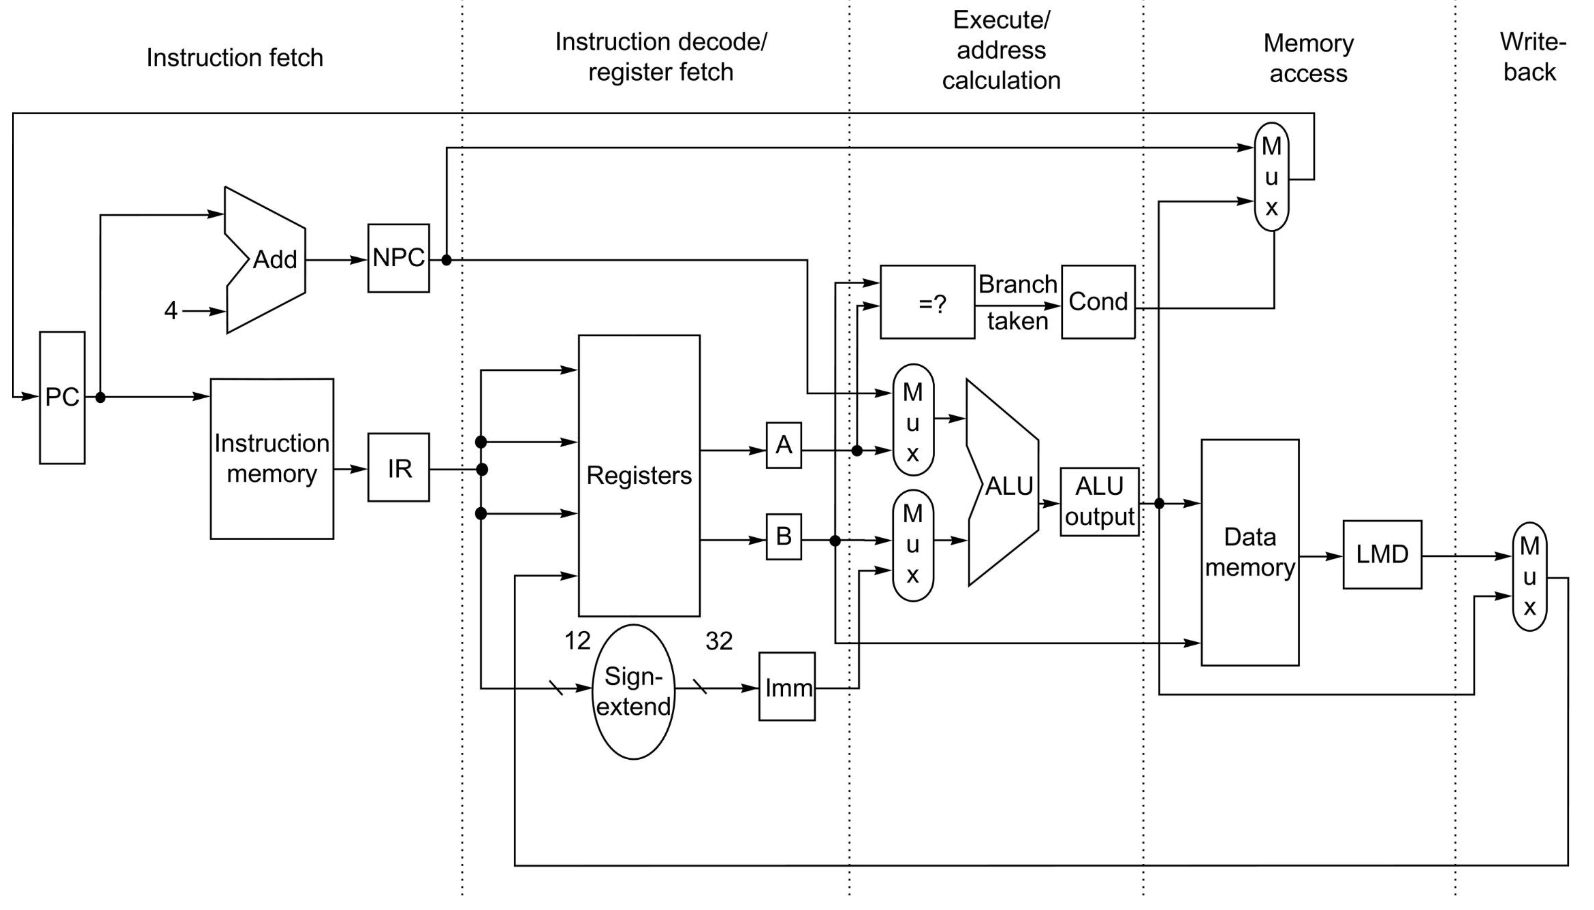
\includegraphics[width=0.9\textwidth]{capitoli/05_pipelining_base/images/datapath_unpipelined.png}
    \caption{Datapath dell'architettura unpipelined, organizzato in 5 fasi logiche.}
    \label{fig:datapath_unpipelined}
\end{figure}

\begin{example}[Valutazione delle prestazioni - Unpipelined vs Pipelined]
    Consideriamo un processore non pipeline con un ciclo di clock di $1\text{ ns}$. Supponiamo che:
    \begin{itemize}
        \item Operazioni ALU e Branch impieghino $4$ cicli (frequenza: $40\% + 20\% = 60\%$).
        \item Operazioni di Memoria impieghino $5$ cicli (frequenza: $40\%$).
    \end{itemize}
    Il tempo di esecuzione medio di un'istruzione si calcola come:
    \[
    \text{Tempo Medio} = \text{Clock Period} \times \text{CPI}_{\text{medio}} = 1\text{ ns} \times ((0.6) \times 4 + (0.4) \times 5) = 1\text{ ns} \times 4.4 = 4.4\text{ ns}
    \]
    Passando a un'architettura pipelined, introduciamo un overhead (ad es. ritardi dei registri). Se questo rallenta il clock del $20\%$, il nuovo clock sarà $1.2\text{ ns}$. Nel caso ideale (un'istruzione completata per ogni ciclo), il tempo medio di esecuzione sarà proprio $1.2\text{ ns}$.
    Lo speedup ottenuto sarà:
    \[
    \text{Speedup} = \frac{4.4\text{ ns}}{1.2\text{ ns}} \approx 3.7 \text{ volte}
    \]
\end{example}

\section{Transizione all'Architettura Pipelined}
Per far sì che l'architettura supporti la pipeline, in modo che ogni risorsa lavori su istruzioni diverse nello stesso colpo di clock, sono necessarie alcune modifiche architetturali:
\begin{itemize}
    \item \textbf{Memorie separate}: Bisogna utilizzare memorie (o cache) separate per Istruzioni e Dati, altrimenti si verificherebbero conflitti strutturali quando uno stadio IF tenta di leggere un'istruzione nello stesso momento in cui uno stadio MEM legge o scrive un dato.
    \item \textbf{Gestione del Register File}: Il banco dei registri è usato da due stadi contemporaneamente: in scrittura (dallo stadio WB) e in lettura (dallo stadio ID). Viene gestito scrivendo nella prima metà del ciclo di clock (first half) e leggendo nella seconda metà (second half).
    \item \textbf{Pipeline Registers (Registri di interstadio)}: \`E essenziale inserire dei registri di stato tra uno stadio e l'altro (\texttt{IF/ID}, \texttt{ID/EX}, \texttt{EX/MEM}, \texttt{MEM/WB}) per memorizzare i dati intermedi e propagarli lungo l'esecuzione dell'istruzione nei colpi di clock successivi.
\end{itemize}

% FIGURA DA INSERIRE QUI
% Fonte: Slide 20
% Descrizione: Diagramma del datapath pipelined con i grandi registri grigi che separano i 5 stadi (IF/ID, ID/EX, EX/MEM, MEM/WB).
\begin{figure}[H]
    \centering
    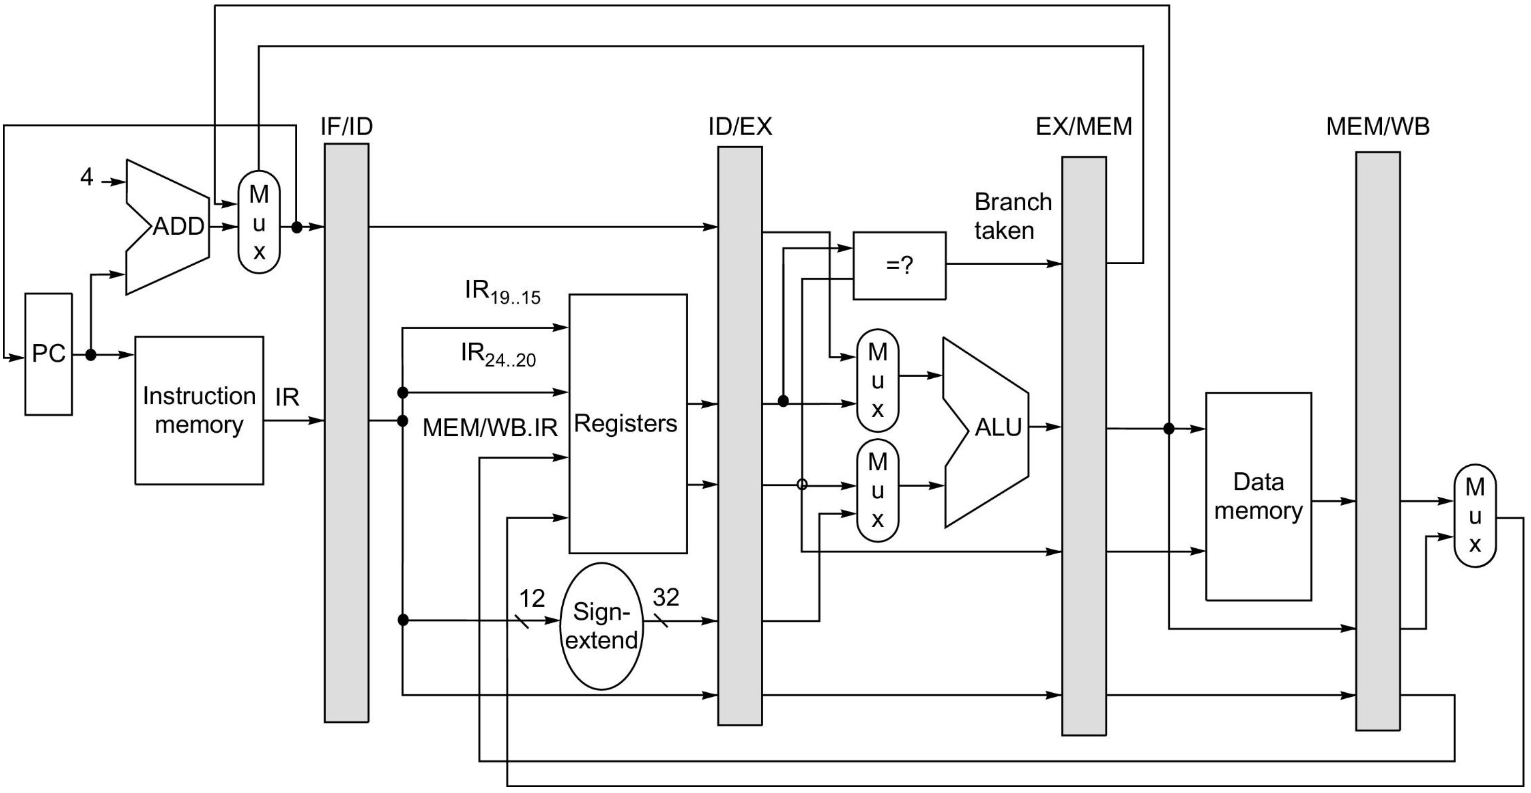
\includegraphics[width=0.9\textwidth]{capitoli/05_pipelining_base/images/datapath_pipelined.png}
    \caption{Datapath pipelined con l'introduzione dei registri di separazione tra gli stadi.}
    \label{fig:datapath_pipelined}
\end{figure}

% FIGURA DA INSERIRE QUI
% Fonte: Slide 21
% Descrizione: Grafico temporale "a cascata" (waterfall) che mostra 5 istruzioni in esecuzione nei cicli di clock, scorrendo diagonalmente da sinistra a destra.
\begin{figure}[H]
    \centering
    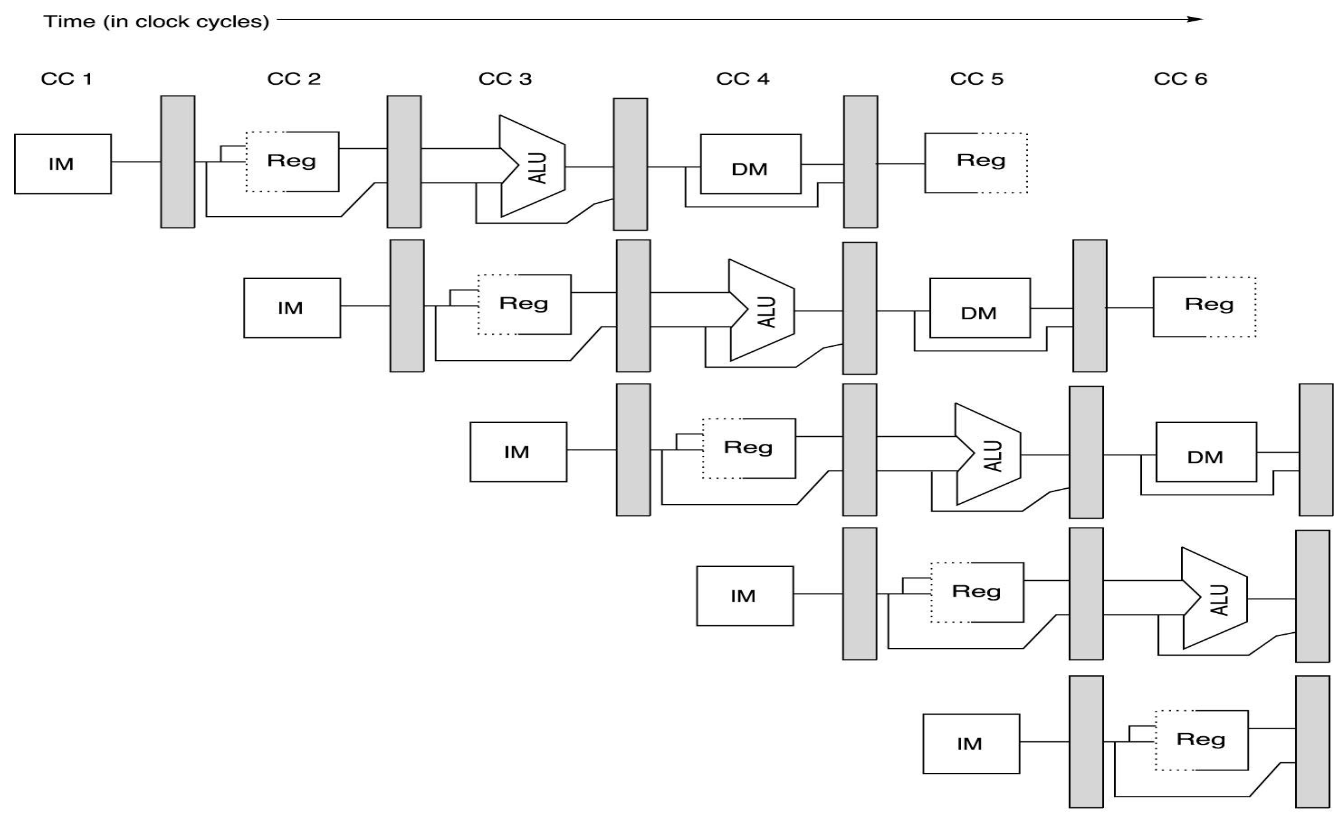
\includegraphics[width=0.9\textwidth]{capitoli/05_pipelining_base/images/evolution_in_time.png}
    \caption{Evoluzione temporale dell'esecuzione pipelined (grafico a cascata).}
    \label{fig:evoluzione_temporale}
\end{figure}

\section{Pipeline Hazards (Conflitti)}
Gli \textbf{Hazards} sono situazioni anomale che impediscono a un'istruzione di essere eseguita nel suo ciclo di clock designato. Non risolti, genererebbero comportamenti non deterministici o risultati errati. 

\subsection{Data Hazards (Conflitti sui Dati)}
La sovrapposizione dell'esecuzione cambia l'ordine con cui si legge e si scrive negli operandi. 
Se un'istruzione necessita del risultato prodotto da un'istruzione immediatamente precedente che non ha ancora raggiunto la fase di Write-Back (WB), si genera un Data Hazard.

\begin{example}
Consideriamo il seguente blocco di codice:
\begin{verbatim}
ADD R1, R2, R3
SUB R4, R1, R5
AND R6, R1, R7
\end{verbatim}
L'istruzione \texttt{ADD} scriverà il valore definitivo nel registro \texttt{R1} solo nello stadio \texttt{WB} (al 5° colpo di clock). L'istruzione \texttt{SUB}, però, entra nella fase \texttt{ID} (lettura dei registri) già al 3° colpo di clock, andando a prelevare un valore di \texttt{R1} obsoleto ed errato.
\end{example}

\subsubsection{Soluzioni ai Data Hazards}
\begin{enumerate}
    \item \textbf{Data Forwarding (Cortocircuitazione)}: Per alcune dipendenze, è possibile prelevare il dato direttamente all'uscita dell'ALU (nello stadio EX o MEM) e iniettarlo direttamente all'ingresso dell'ALU per l'istruzione successiva, anticipando l'attesa del ciclo WB.
    \item \textbf{Stalli (Pipeline Stall o Bubble)}: 
    Come sottolineato dal professore, in certi casi (es. operazione di \texttt{Load} da memoria dove il dato arriva fisicamente alla fine dello stadio MEM), il forwarding non è fisicamente possibile perché si richiederebbe di "mandare il dato indietro nel tempo" rispetto ai colpi di clock (vedi Fig. \ref{fig:stall_bubble}). In questo caso interviene la circuiteria di interlock che inserisce uno \textbf{stallo} (chiamato \textit{bubble} o bolla). 
    La bolla transita per tutti gli stadi successivi, rallentando l'esecuzione dell'istruzione dipendente fintanto che il dato non è disponibile per essere forwardato correttamente.
\end{enumerate}

% FIGURA DA INSERIRE QUI
% Fonte: Slide 52
% Descrizione: Esempio con Forwarding impossibile che va "indietro nel tempo" (curva all'indietro dal DM all'ALU del ciclo precedente) e sua risoluzione tramite stallo/Bubble.
\begin{figure}[H]
    \centering
    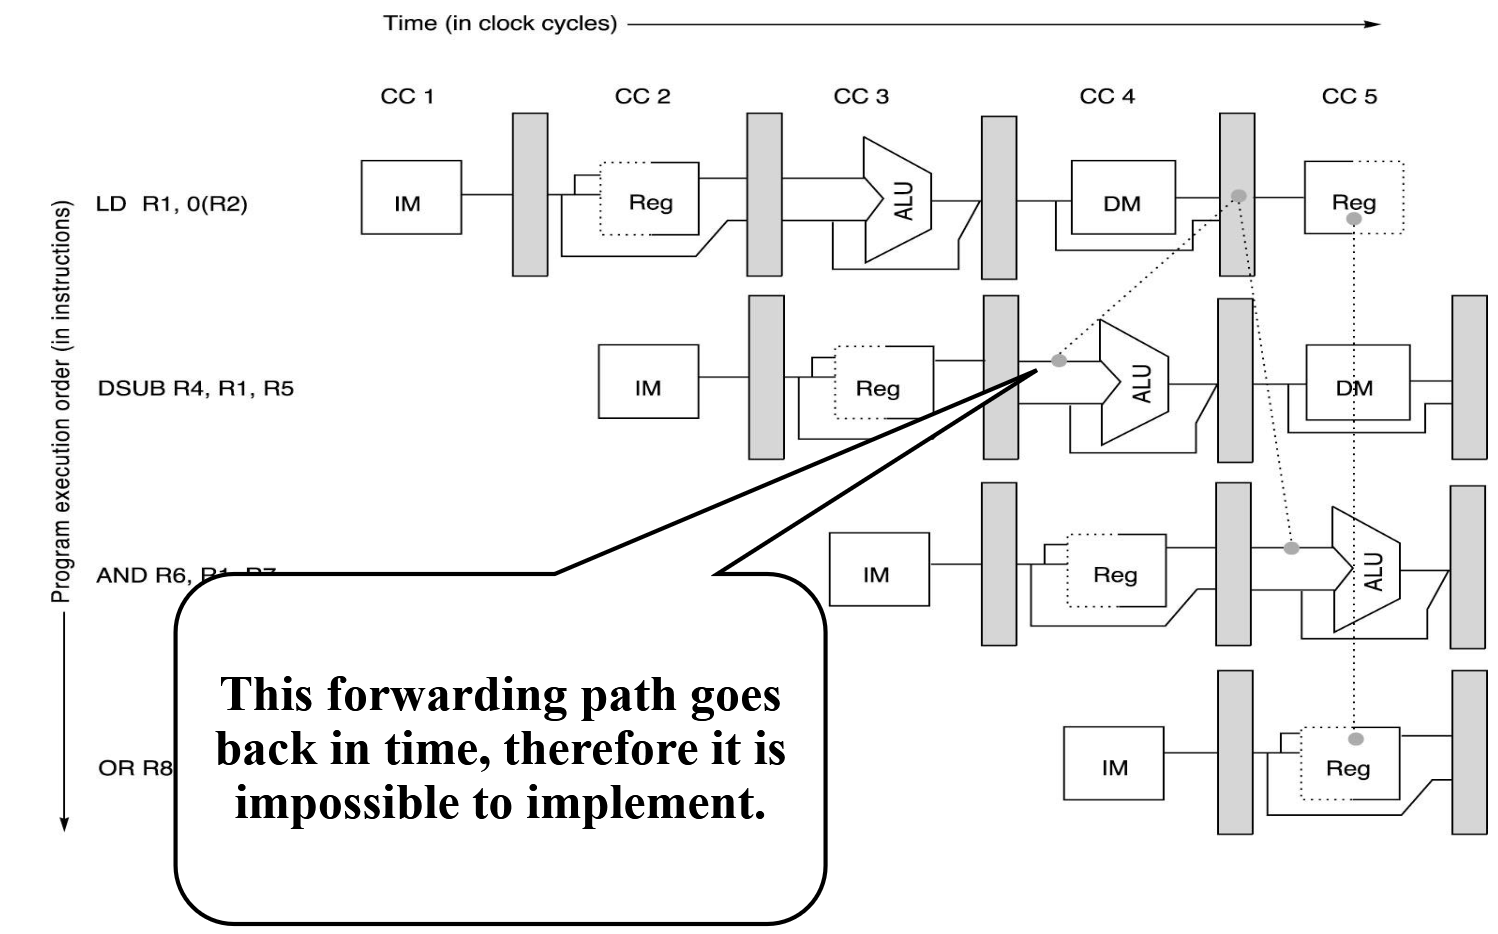
\includegraphics[width=0.6\textwidth]{capitoli/05_pipelining_base/images/impossible_forwarding.png}
    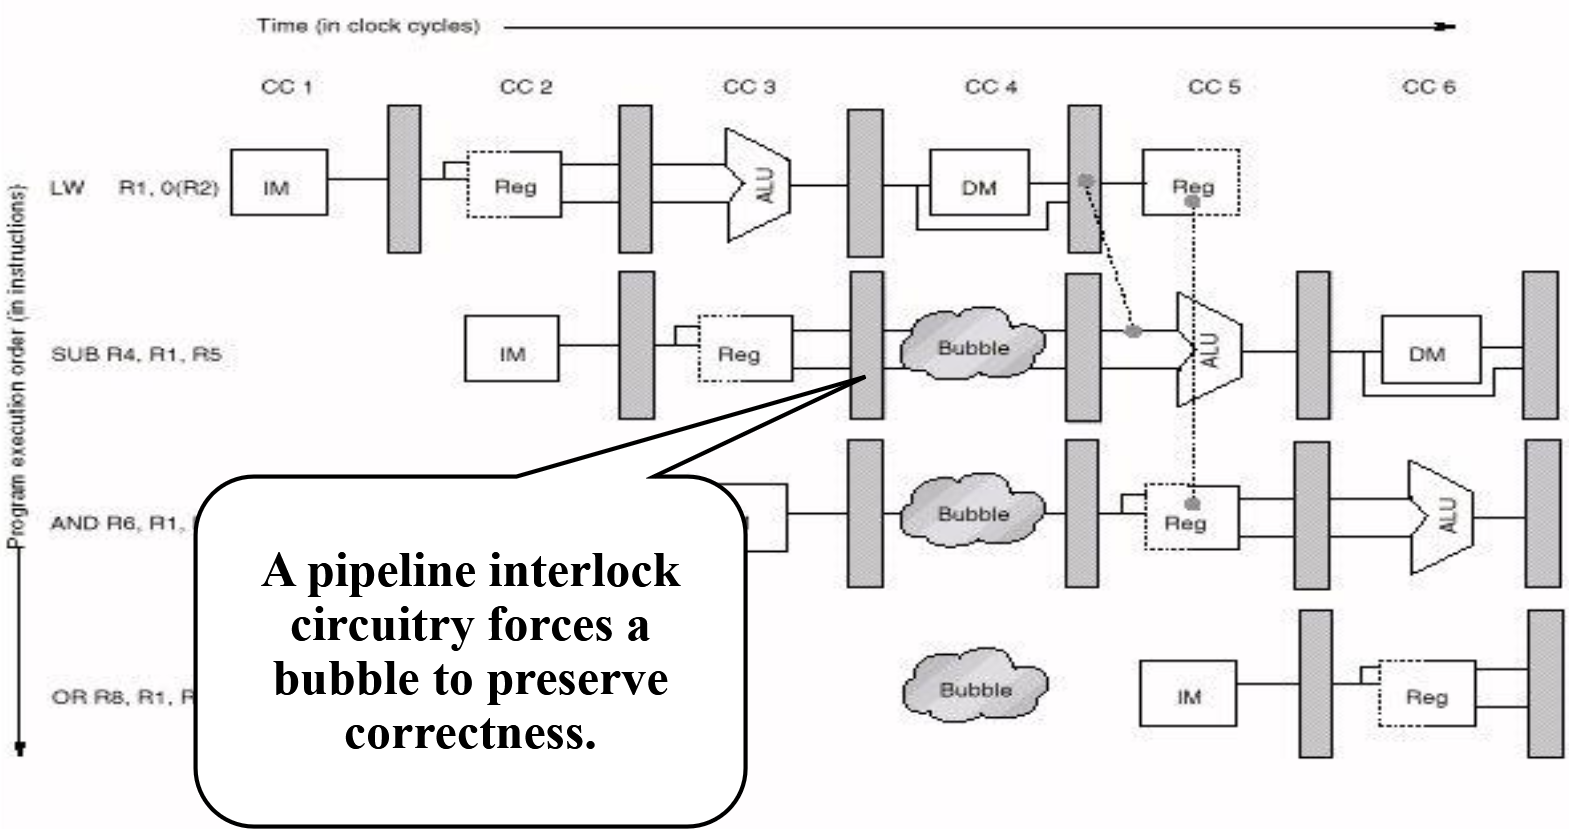
\includegraphics[width=0.6\textwidth]{capitoli/05_pipelining_base/images/bubble_stall.png}
    \caption{Risoluzione di un Load-use Data Hazard inserendo una Bubble (bolla) nella pipeline per ritardare l'istruzione dipendente.}
    \label{fig:stall_bubble}
\end{figure}

\subsection{Control Hazards (Conflitti di Controllo)}
I conflitti di controllo sono dovuti alle istruzioni di salto (\textit{branches}, condizionati o incondizionati). Il problema nasce perché il salto può modificare il Program Counter (\texttt{PC}), ma questa decisione (ovvero capire \textit{se} si salta e \textit{dove} si salta) viene presa quando l'istruzione successiva è già entrata nella pipeline.
Nella versione base della pipeline, il target del PC viene scritto alla fine dello stadio \texttt{EX} (ovvero $2$ colpi di clock dopo la fase IF in cui il branch è stato caricato), obbligando il processore ad annullare ben due istruzioni successive già processate se il salto è \textit{preso} (taken).

\begin{figure}[H]
    \centering
    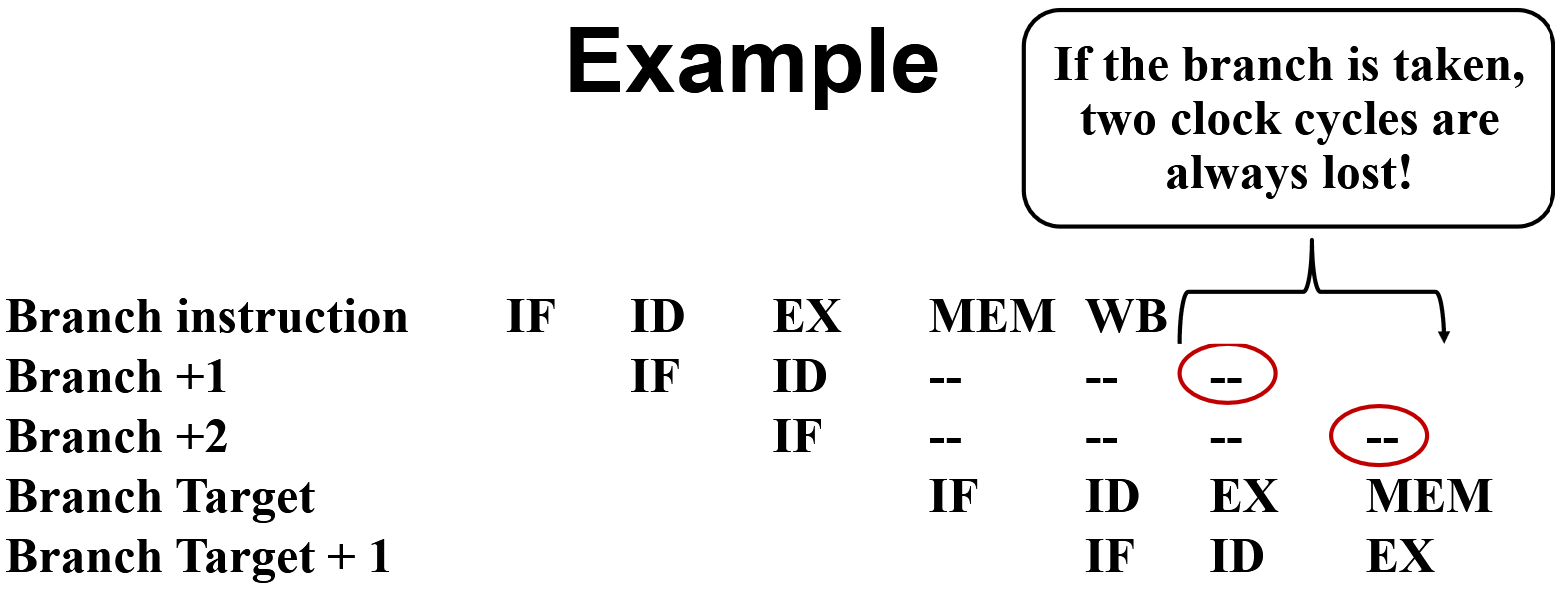
\includegraphics[width=0.6\textwidth]{capitoli/05_pipelining_base/images/lost_cycles.png}
    \caption{Esempio di Control Hazard: se il branch è preso, le due istruzioni successive vengono annullate, causando una perdita di cicli di clock.}
    \label{fig:lost_cycles}
\end{figure}

\subsubsection{Soluzioni ai Control Hazards}
\begin{itemize}
    \item \textbf{Anticipazione (Basic Solution)}: La circuiteria del branch viene spostata nello stadio \textbf{ID}. Si anticipa quindi sia la decisione se saltare, sia il calcolo del target \texttt{PC}. Lo stallo viene ridotto, ma si inserisce hardware aggiuntivo nel datapath in fase ID.
    \item \textbf{Delayed Branch (Salto ritardato)}: Il compilatore inserisce nel \textit{delay slot} (lo spazio temporale subito dopo il branch) istruzioni indipendenti e sicure da eseguire, indipendentemente dall'esito del salto. 
    \begin{remark}[Evoluzione tecnologica]
    Oggi questa tecnica è diventata obsoleta. Con l'avvento di processori con \textit{deep pipeline} (pipeline molto profonde, anche da 15-20 stadi), la lunghezza dei delay slot aumenta vistosamente, rendendo quasi impossibile per il compilatore trovare abbastanza istruzioni utili per riempirli. Pertanto, gran parte delle moderne architetture RISC non li supporta più, preferendo meccanismi complessi di \textit{Branch Prediction} (previsione di salto).
    \end{remark}
\end{itemize}

% FIGURA DA INSERIRE QUI
% Fonte: Slide 63
% Descrizione: Datapath con anticipazione della logica di salto (calcolo target PC e comparazione) inserita nello stadio ID/EX, con evidenziatori rossi sulla nuova circuiteria.
\begin{figure}[H]
    \centering
    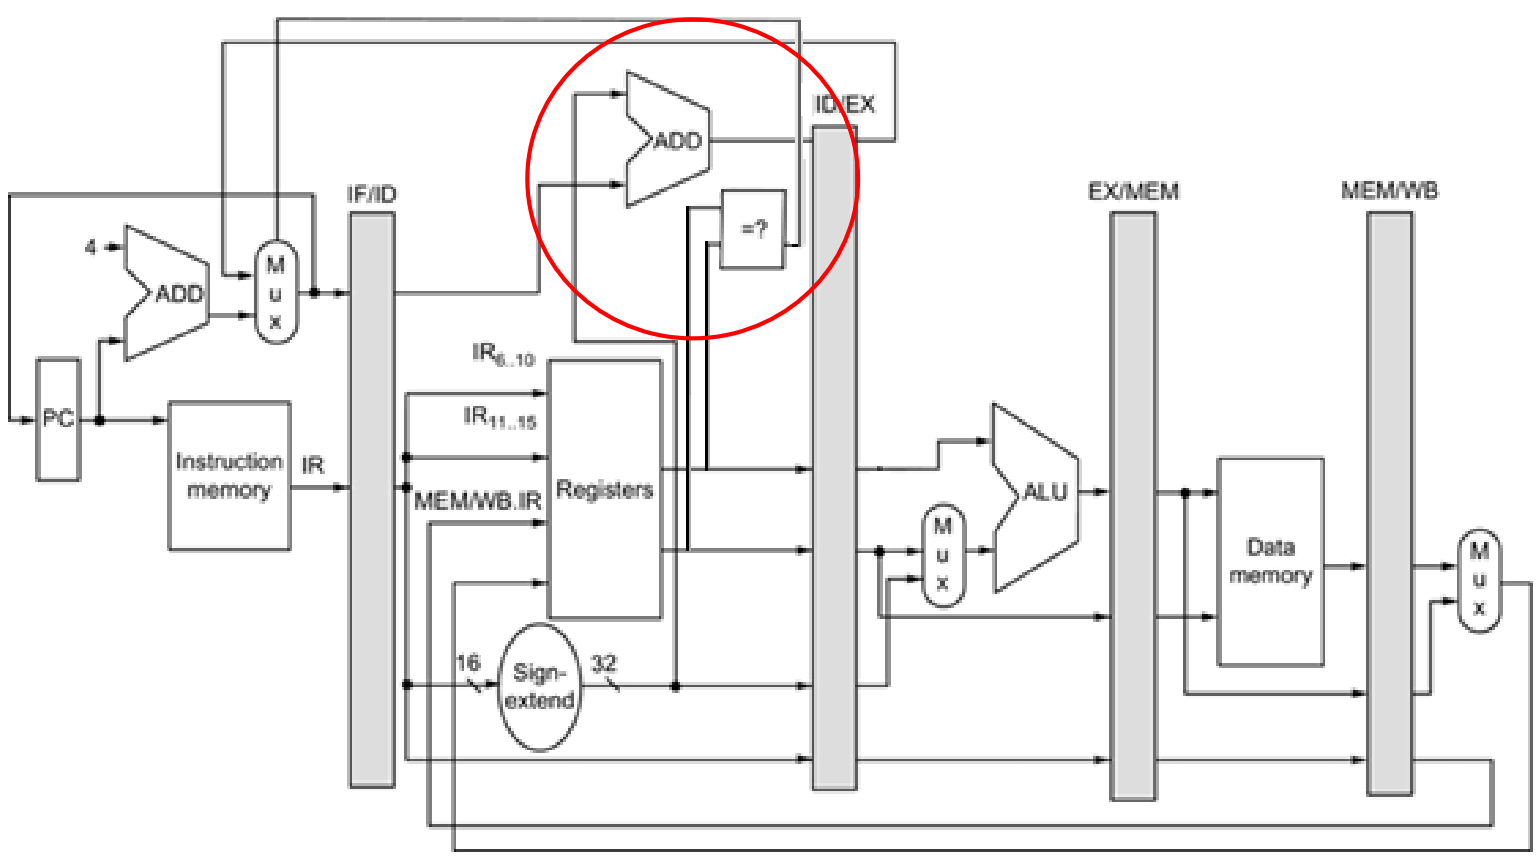
\includegraphics[width=0.6\textwidth]{capitoli/05_pipelining_base/images/early_branch.png}
    \caption{Spostamento della logica di salto (calcolo dell'indirizzo e confronto) nello stadio ID per mitigare la penalty da control hazard.}
    \label{fig:early_branch}
\end{figure}